Based on the compartmental model and parameters published by Rivers et al.\cite{Rivers2014} in October 2014, it was modeled a similar approach in Insight Maker.  This particular model, divides the population into six different compartments; the Susceptible persons (S) could become Exposed (E), if they were in contact with an infected individual, initiating a transition to the Infectious (I) state after the incubation period of the disease, subsequently, acquiring the capacity of infecting others. A percentage of the I class individuals may be Hospitalized (H). There are two possible outcomes for the untreated individuals in I and the treated patients in H, individuals may die, with a probability of infecting other people during the resultant Funeral (F), before the virus is removed (R) from the individual, or the patients may recover, at this stage, can be considered equivalently removed. However,  in order to distinguish between the recovered (R) patients and the deceased (D) individuals, was considered a model with seven compartments : S, E, I, H, F, R and D. Figure ~\ref{fig:compartment} depicts the implemented compartment model. \\



\begin{figure}[!h]
  \centering
  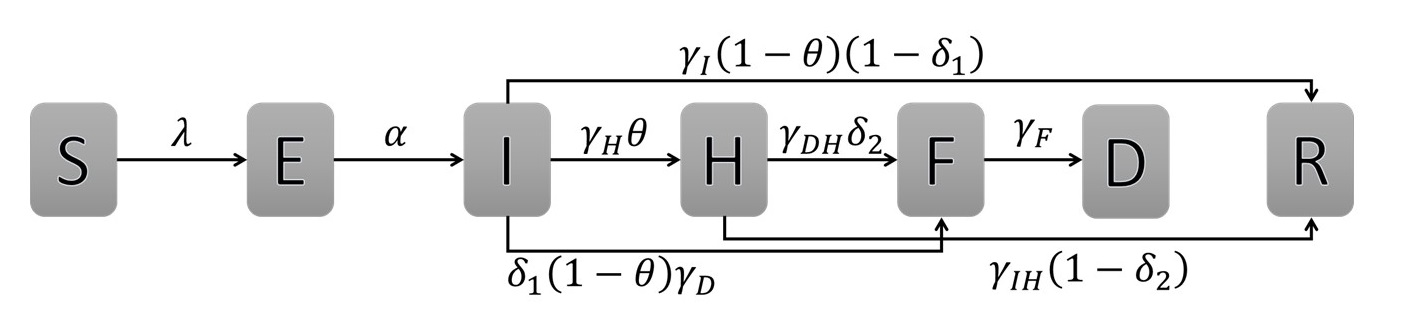
\includegraphics[width=1\textwidth]{compartment}
  \caption{Compartment Model of the Ebola Epidemic in Liberia. \newline  Being S: Susceptible, E: Exposed, I: Infectious, H: Hospitalized, F: Funeral,  R: Recovered and D: Dead. All the possible flows are specified by the arrows and the parameters that direct them. Note that $\lambda = \beta_{I}I+\beta_{H}H+\beta_{F}F $, is a combination of all the $\beta$ transmission terms shown in Table~\ref{tab:parameters} } 
\label{fig:compartment} 
\end{figure}

 
The governing equations of the system dynamics described above are the following:
\begin{eqnarray} 
\label{SDeqn}
\frac{dS}{dt} = - \frac{\beta_{I}SI+\beta_{H}SH+\beta_{F}SF}{N}\\
\frac{dE}{dt} =  \frac{\beta_{I}SI+\beta_{H}SH+\beta_{F}SF}{N}-\alpha E\\
\frac{dI}{dt} =  \alpha E - [\gamma_{H}\theta + \gamma_{I}(1-\theta)(1-\delta_{1})+\gamma_{D}(1-\theta)\delta_{1}]I\\
\frac{dH}{dt} = \gamma_{H}\theta I - [\gamma_{DH}\delta_{2}+\gamma_{IH}(1-\delta_{2})]H\\
\frac{dF}{dt} = \gamma_{D}(1-\theta) \delta_{1} I + \gamma_{DH}\delta_{2} H-\gamma_{F} F\\
\frac{dR}{dt} = \gamma_{I}(1-\theta)(1- \delta_{1}) I + \gamma_{IH}(1-\delta_{2}) H-\gamma_{F} F
\end{eqnarray}
where each of the parameters are defined on Table \ref{tab:parameters}


%INSIGHT MAKER DESCRIPTION AND RESULTS
\subsection{Insight Maker}
 Insight Maker is a powerful online tool used to model and simulate complex systems. It utilizes different approaches, such as System Dynamics, Agent-Based Modeling and imperative programming. Insight Makera construction of a graphical model to forecast the system response \cite{FortmannRoe}. We used the InsightMaker platform to prototype our model and simulate stepping forward through time. More details about the platform and its functionality can be found in Fortmann-Roe's review \cite{FortmannRoe}. The platform uses a fourth order Runge-Kutta differential equation solver for the system dynamics model and  first order Euler approximation for the Agent-Based model.

\noindent The implemented Insight Maker SD model is depicted in Figure \ref{fig:SD_IM} .


\begin{figure}[!h]
  \centering
  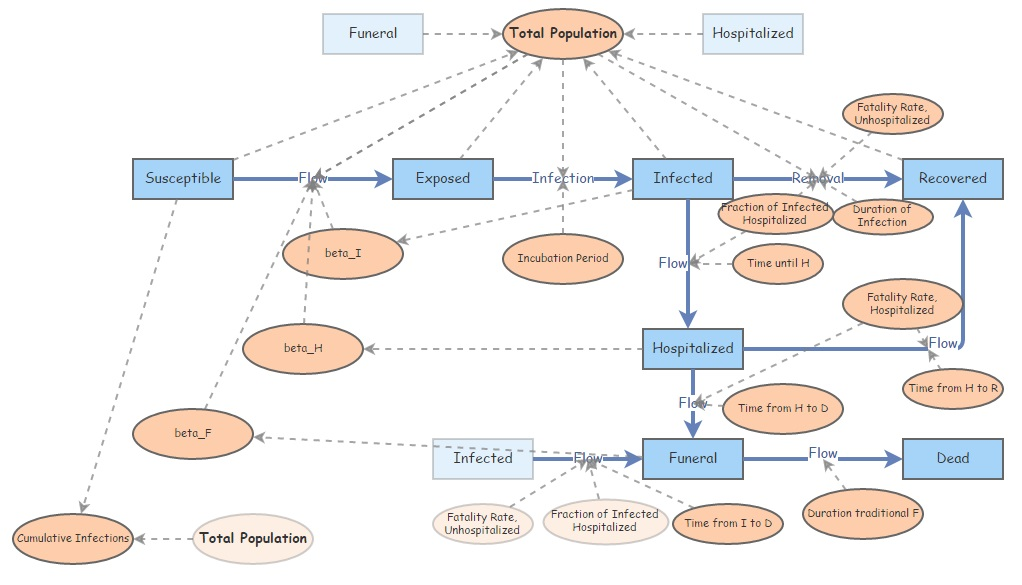
\includegraphics[width=1\textwidth]{SD_IM}
  \caption{ Compartment model of the system dynamics implemented on Insight Maker}
\label{fig:SD_IM} 
\end{figure}

\noindent A normalized population fraction was simulated. The compartment S was initialized with a value of 999.999/1.000.000, and the compartment I with 1/1.000.000, meaning that there is an infected individual per every million of individuals, the rest of the compartments were set to zero as an initial condition. The flow between the compartments is specified in Figure \ref{fig:compartment.} and all the other parameters were initialized as shown in Table \ref{tab:parameters}.  As mention in Section \ref{sec:calibration}, the parameters were calibrated in two stages, before and after the international intervention. According with the time frame proposed, the change in the parameters was also implemented on Insight Maker. The links to the online models can be found on \cite{IM_AI} and  \cite{IM_BI}.  


% RESULTS AND DISCUSSION
%
%No intervention
\noindent After modeling the system with the parameters before the intervention, it can be observed in Figure \ref{fig:LB_IM_NoIn} how the total population decreases to 46.46\%  if there is no intervention and the each of the parameters continue to be the same. The number of susceptible individuals exponentially decays, converging to 7\% of the population, while exposed, infected, hospitalized and funeral comparments converges to zero; finally, after the system stabilizes, the final proportion of deaths would be 53.53\% 

\begin{figure}[!h]
  \centering
  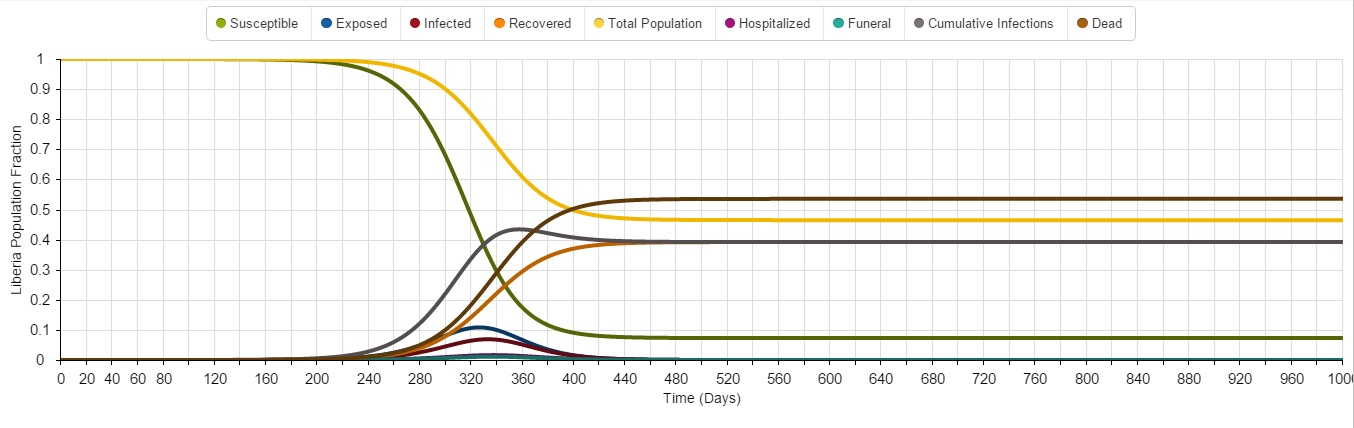
\includegraphics[width=1\textwidth]{LB_NoInt_SD_IM}
  \caption{ Insight Maker results using the parameters of the first stage (Mar/14 to Sept/14) and assuming no intervention}
\label{fig:LB_IM_NoIn} 
\end{figure}

%Intervention 
\noindent As mentioned before, five parameters were calibrated for the second stage of the Ebola Outbreak, namely, community contact rate ($\beta_I$), hospital contact rate ($\beta_H$), funeral contact rate ($\beta_F$), time until hospitalization ($\gamma_H$) and probability a case is hospitalized ($\theta$). Figure \ref{fig:LB_IM_In} A. shows that there is not much change in the Total population and susceptible compartment, meaning that the virus was controlled;  Figure \ref{fig:LB_IM_In} B focuses on E, I, R, H , F and D compartments, showing that the international intervention causes a dramatic change in the behavior of such compartments.

\begin{figure}[!h]
  \centering
  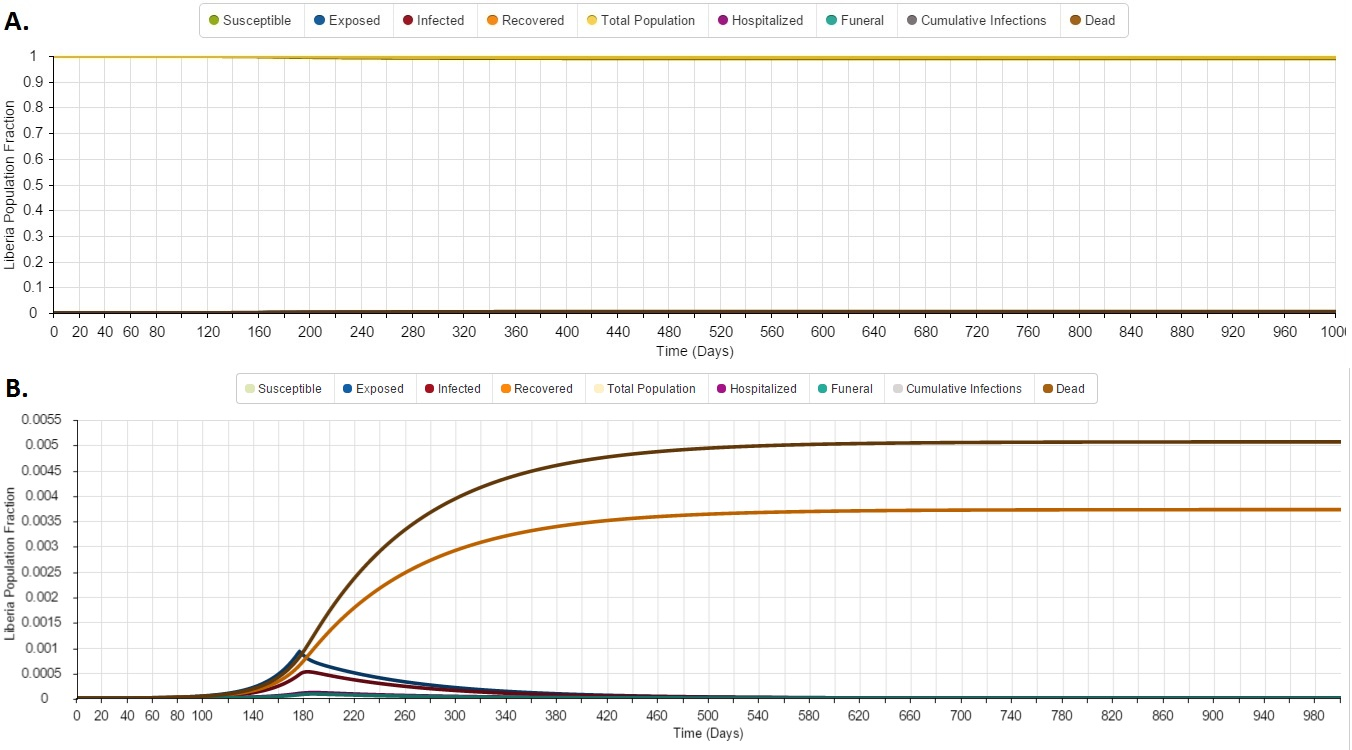
\includegraphics[width=1\textwidth]{LB_Int3_SD_IM}
  \caption{ Insight Maker results. \textit{A.} Parameters of the first stage (Mar/14 to Sept/14), \textit{B.} Parameters of the second stage ( Sept/14 to July/15)}
\label{fig:LB_IM_In} 
\end{figure}


%Comparing with WHO data

\noindent Finally, a comparison between the proposed model and World Health Organization data is shown in Figures \ref{fig:LB_IM_WHO} and \ref{fig:LB_IM_WHO2}. As depicted in Figure \ref{fig:LB_IM_WHO} A and B there is a good fitting of our model with the data reported by WHO. Figure \ref{fig:LB_IM_WHO2} shows  the reported WHO data before and after intervention, the results of our model before and after intervention and the forecast for the coming months, predicting that after the system reaches an equilibrium, the proportion of deaths in Liberia product of the EVD would be 5.07\% approximately.


\begin{figure}[!h]
  \centering
  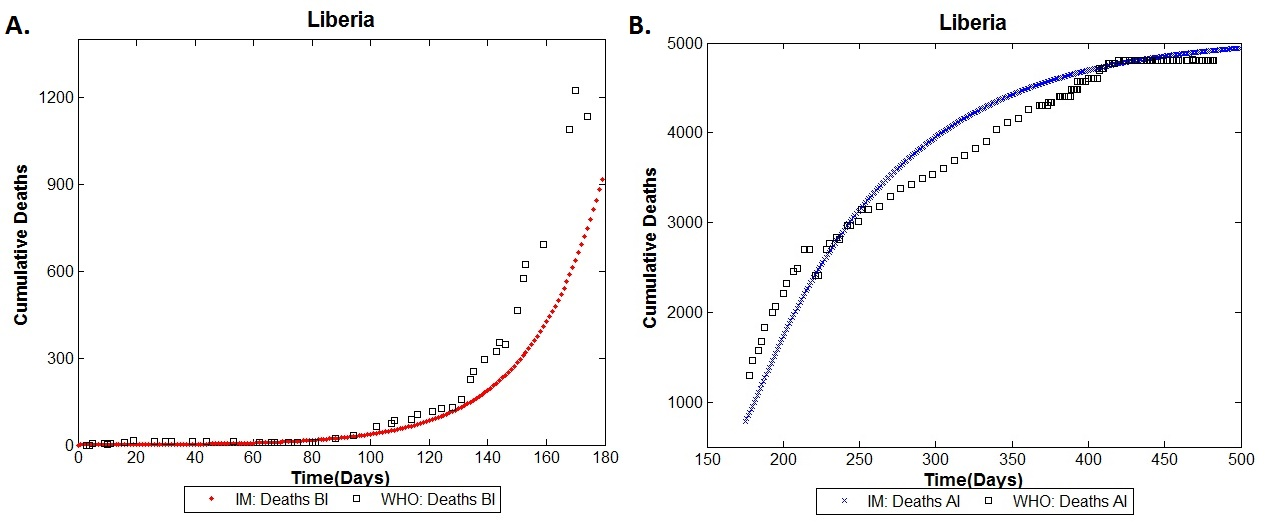
\includegraphics[width=1\textwidth]{LB_BI_AI_SD_WHO_IM}
  \caption{ Comparison between World Health Organization (WHO) data and Insight Maker (IM) results using the parameters of A. the first stage (Mar/14 to Sept/14) and B. the second stage ( Sept/14 to July/15) for the cumulative deaths (D).}
\label{fig:LB_IM_WHO} 
\end{figure}



\begin{figure}[!h]
  \centering
  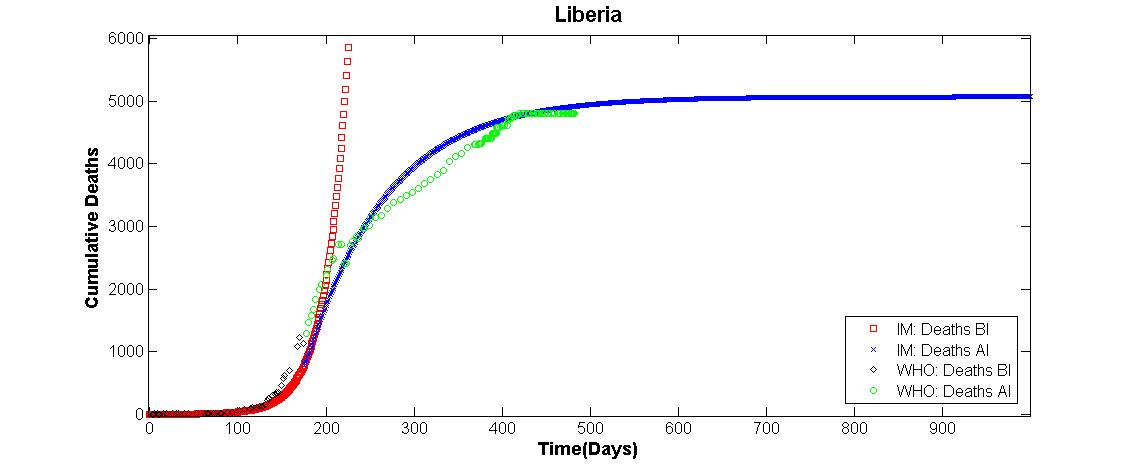
\includegraphics[width=1\textwidth]{LB_Int2_SD_WHO_IM}
  \caption{ Comparison between World Health Organization (WHO) data and Insight Maker (IM) results using the parameters before intervention (BI) and after intervention (AI), for the cumulative deaths (D).}
\label{fig:LB_IM_WHO2} 
\end{figure}


%%MATHEMATICA DESCRIPTION
\newpage
\subsection{Mathematica}
We drew the plots in the previous section also with Mathematica, and got almost same result. One additional plot we draw in Mathematica is phase portrait of the system (Figure).

\begin{figure}[!h]
  \centering
  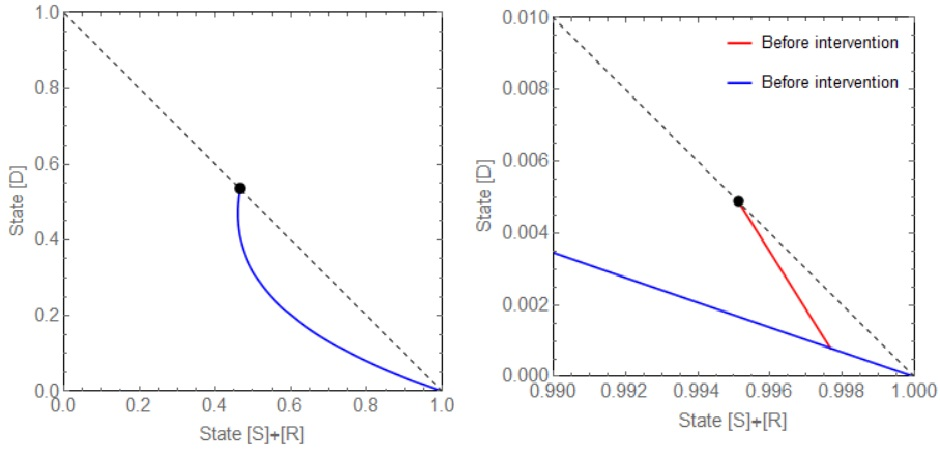
\includegraphics[width=1\textwidth]{PhasePortrait}
  \caption{Projection of phase portrait to (Susceptible + Recovered, Dead) space. (Blue) - without intervention, (Red) - with intervention, (Dots) - where the phase converges (equilibrium).}
\label{fig:Phase Portrait}
\end{figure}
